\subsection{Modifica test salvato}

\begin{figure}[H]
    \centering
    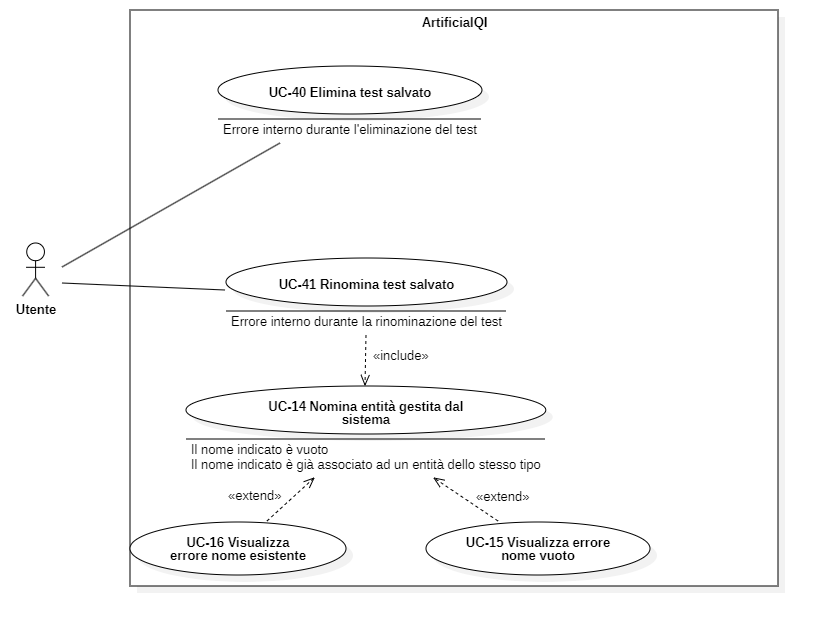
\includegraphics[scale=0.2]{Sezioni/UseCase/Immagini/ModificaTestSalvato.png}
    \caption{Diagramma per la Modifica di un test salvato.}
\end{figure}

\begin{usecase}{UC-43}{Elimina test salvato}
    \label{uc:UC-43}
    
    \req{\hyperref[ru:RUF-1]{RUF-1}}
    
    \pre{
        \item L'utente sta visualizzando i test salvati
        \item Il test da eliminare esiste
    }
    
    \post{
        \item Il test salvato viene eliminato
    }
    
    \actor{
        Utente
    }
    
    \subactors{}
    
    \trigger{L'utente vuole eliminare un test salvato}
    
    \inc{}
    
    \base{}
    
    \scenario{
        \item L'utente richiede di eliminare un test salvato
        \item L'utente conferma l'eliminazione
        \item Il sistema elimina il test 
        \item Il sistema notifica l'utente della corretta eliminazione
    }
    
    \subscenario{
        \item[2.1] L'utente annulla l'eliminazione:
        \begin{itemize}
            \item Il sistema annulla l'operazione
        \end{itemize}
        \item[3.1] Avviene un errore interno durante l'eliminazione del test:
        \begin{itemize}
            \item \hyperref[uc:UC-16]{UC-16}
        \end{itemize}
    }

\end{usecase}

\begin{usecase}{UC-44}{Rinomina test salvato}
    \label{uc:UC-44}
    
    \req{\hyperref[ru:RUF-1]{RUF-1}}
    
    \pre{
        \item L'utente sta visualizzando i test salvati
        \item Il test da rinominare esiste
    }
    
    \post{
        \item Il test salvato viene rinominato
    }
    
    \actor{
        Utente
    }
    
    \subactors{}
    
    \trigger{L'utente vuole rinominare un test salvato}
    
    \inc{\hyperref[uc:UC-17]{UC-17}}
    
    \base{}
    
    \scenario{
        \item L'utente richiede di rinominare un test salvato
        \item Il sistema ottiene il nuovo nome per il test seguendo \hyperref[uc:UC-17]{UC-17}
        \item L'utente conferma la rinominazione
        \item Il sistema rinomina il test
        \item Il sistema notifica l'utente della corretta rinominazione
    }
    
    \subscenario{
        \item[3.1] L'utente annulla la rinominazione:
        \begin{itemize}
            \item Il sistema annulla l'operazione
        \end{itemize}
        \item[4.1] Avviene un errore interno durante la rinominazione del test:
        \begin{itemize}
            \item \hyperref[uc:UC-16]{UC-16}
        \end{itemize}
    }

\end{usecase}